\chapter{Transformações que não podem ser desfeitas}\label{ch:g5:irreversible-changes}

Um ovo é quebrado numa frigideira quente. Em poucos segundos, a clara
transparente e mole fica firme e branca, e a gema engrossa. Tire a
frigideira do fogão, deixe o ovo esfriar, ponha-o na geladeira: ele
nunca mais vai ser um ovo cru. Algumas transformações podem ser
desfeitas e outras não. Distinguir umas das outras é o primeiro passo da
química.

\begin{recall}
Um sólido que \omterm{def:g2:mixing-and-dissolving:dissolve}{se dissolve} na água continua lá: quando a água seca, o
sólido fica para trás (\cref{ch:g2:mixing-and-dissolving}). Uma \omterm{def:g4:what-a-fire-needs:burning}{queima}
fabrica substâncias novas --- cinza, fumaça, dióxido de carbono, vapor
de água --- e o \omterm{def:g4:what-a-fire-needs:fuel}{combustível} acaba para sempre
(\cref{ch:g4:what-a-fire-needs}).
\end{recall}

\begin{omfigure}
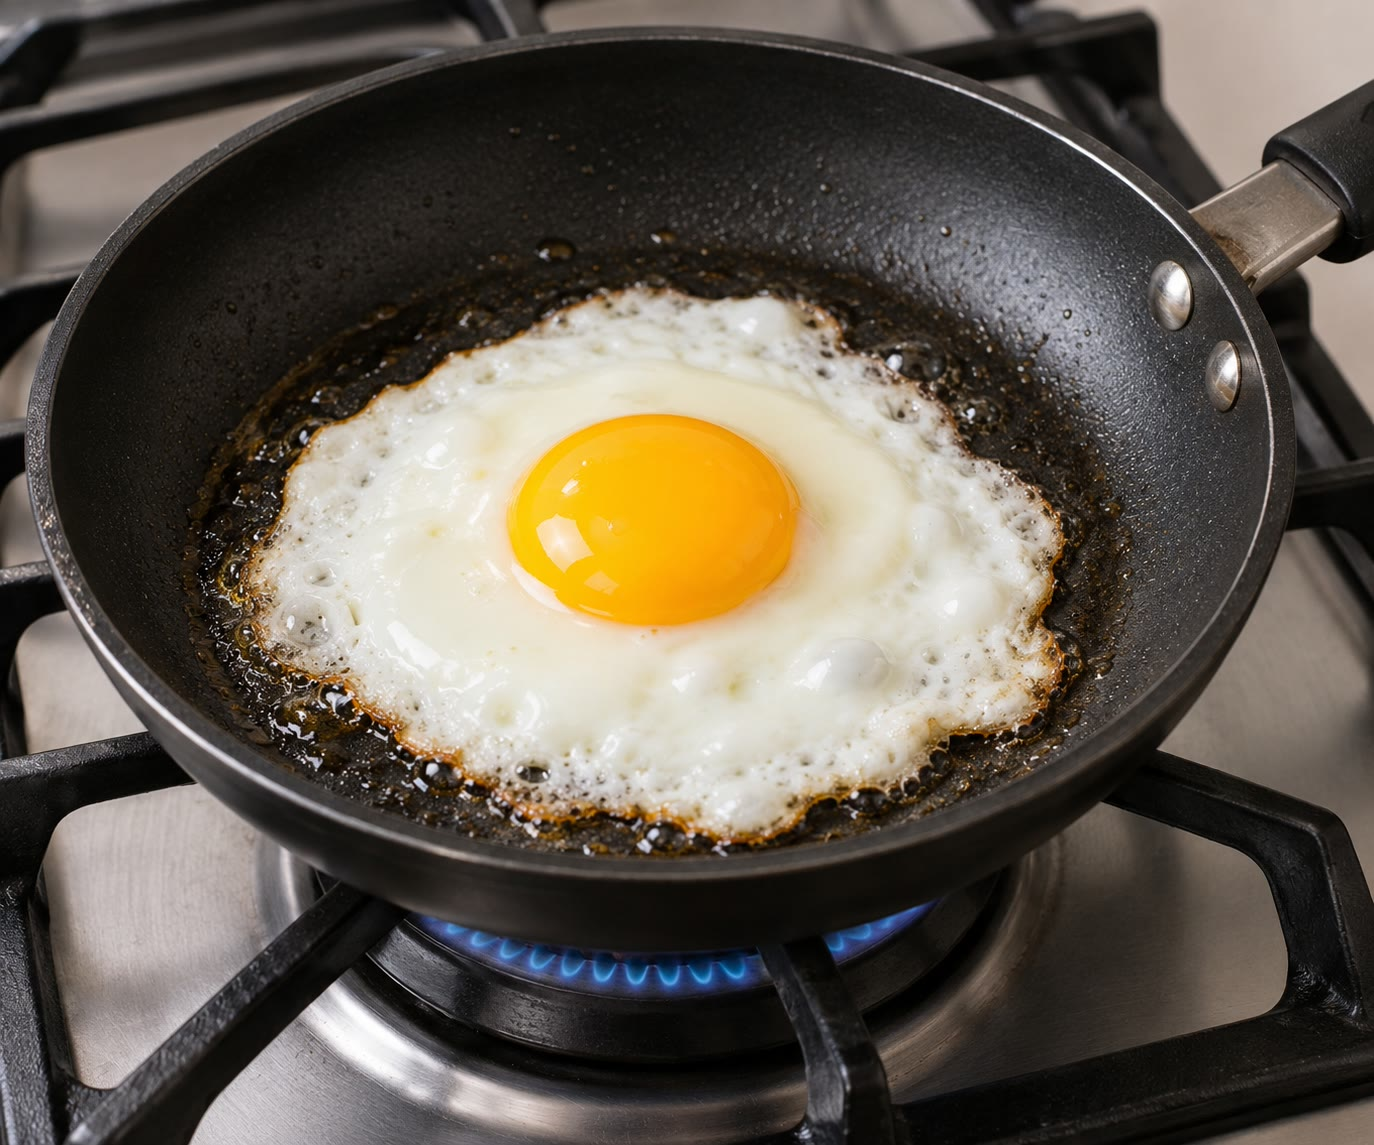
\includegraphics[width=0.55\linewidth]{images/book1/ai/g5-egg-frying.jpg}

{\small Um ovo fritando: a clara transparente ficou firme e branca, para
sempre.}
\end{omfigure}

\section{Transformações que podem ser desfeitas}

\begin{definition}[Transformação reversível]\label{def:g5:irreversible-changes:reversible}
Uma \emph{transformação reversível}\index{transformacao reversivel@transformação reversível} é uma
transformação que pode ser desfeita, de modo que recuperamos exatamente
o que tínhamos no começo.
\end{definition}

\begin{example}[Dissolver e secar]\label{ex:g5:irreversible-changes:dissolve}
O açúcar mexido na água \omterm{def:g2:mixing-and-dissolving:dissolve}{se dissolve}. Deixe a água evaporar, e o açúcar
volta: o mesmo açúcar, doce como antes. \omterm{def:g2:mixing-and-dissolving:dissolve}{Dissolver} é uma \omterm{def:g5:irreversible-changes:reversible}{transformação
reversível}.
\end{example}

\begin{example}[Gelo e água]\label{ex:g5:irreversible-changes:ice}
Um cubo de gelo derrete e vira água num prato morno; ponha a água no
congelador e ela vira gelo de novo. Derreter e congelar são
\omterm{def:g5:irreversible-changes:reversible}{transformações reversíveis}. (Por que a água derrete e congela é contado
no livro de física.)
\end{example}

\begin{example}[Misturar]\label{ex:g5:irreversible-changes:mix}
A areia \omterm{def:g2:mixing-and-dissolving:mix}{misturada} com cascalho pode ser separada de novo com uma
peneira; a água barrenta pode ser filtrada. \omterm{def:g2:mixing-and-dissolving:mix}{Misturar} é uma \omterm{def:g5:irreversible-changes:reversible}{transformação
reversível}: nada de novo é fabricado, e as partes podem ser separadas
(\cref{ch:g3:separating-mixtures}).
\end{example}

\section{Transformações que não podem ser desfeitas}

\begin{definition}[Transformação irreversível e transformação química]\label{def:g5:irreversible-changes:chemical-change}
Uma \emph{transformação irreversível}\index{transformacao irreversivel@transformação irreversível} é
uma transformação que não pode ser desfeita de um jeito simples. A
maioria delas são transformações em que aparecem substâncias novas, que
não estavam lá no começo: uma transformação assim se chama
\emph{transformação química}\index{transformacao quimica@transformação química}.
\end{definition}

\begin{example}[Seis transformações químicas]\label{ex:g5:irreversible-changes:six}
\begin{itemize}
  \item \textbf{Cozinhar um ovo}: a clara mole e transparente fica firme
        e branca.
  \item \textbf{Assar um bolo}: uma massa mole vira um bolo fofo, dourado
        por fora, com um cheiro novo.
  \item \textbf{Queimar}: a madeira vira cinza, fumaça, dióxido de
        carbono e vapor de água.
  \item \textbf{Enferrujar}: o ferro brilhante deixado na chuva fica
        coberto por uma substância marrom-alaranjada que se esfarela, a
        ferrugem.
  \item \textbf{O leite azedar}: esquecido por dias, o leite engrossa,
        forma grumos e fica com cheiro azedo.
  \item \textbf{Uma maçã cortada escurecer}: a polpa clara fica marrom no
        \omterm{def:g4:air-a-mixture-of-gases:air}{ar} em menos de uma hora.
\end{itemize}
Em cada caso foi fabricada uma coisa nova, e não há um jeito simples de
recuperar o que tínhamos no começo.
\end{example}

\begin{omfigure}
\begin{minipage}[t]{0.48\linewidth}\centering
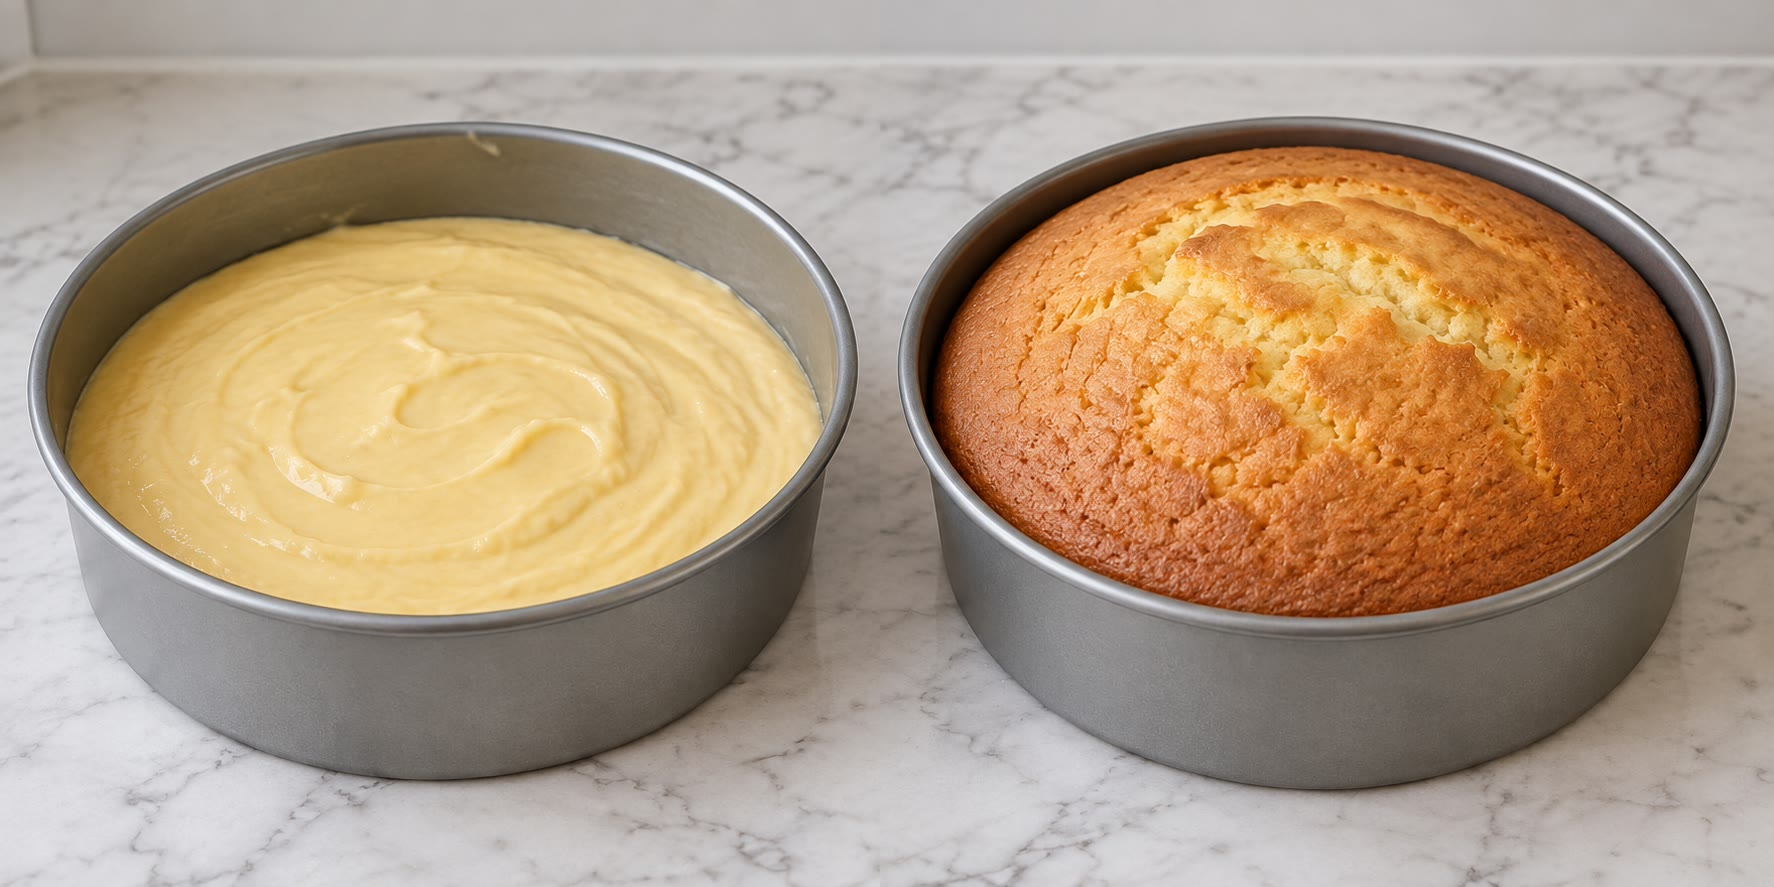
\includegraphics[width=\linewidth,height=4.6cm,keepaspectratio]{images/book1/ai/g5-cake-before-after.jpg}

{\small A massa antes, o bolo depois: assar não pode ser desfeito.}
\end{minipage}\hfill
\begin{minipage}[t]{0.48\linewidth}\centering
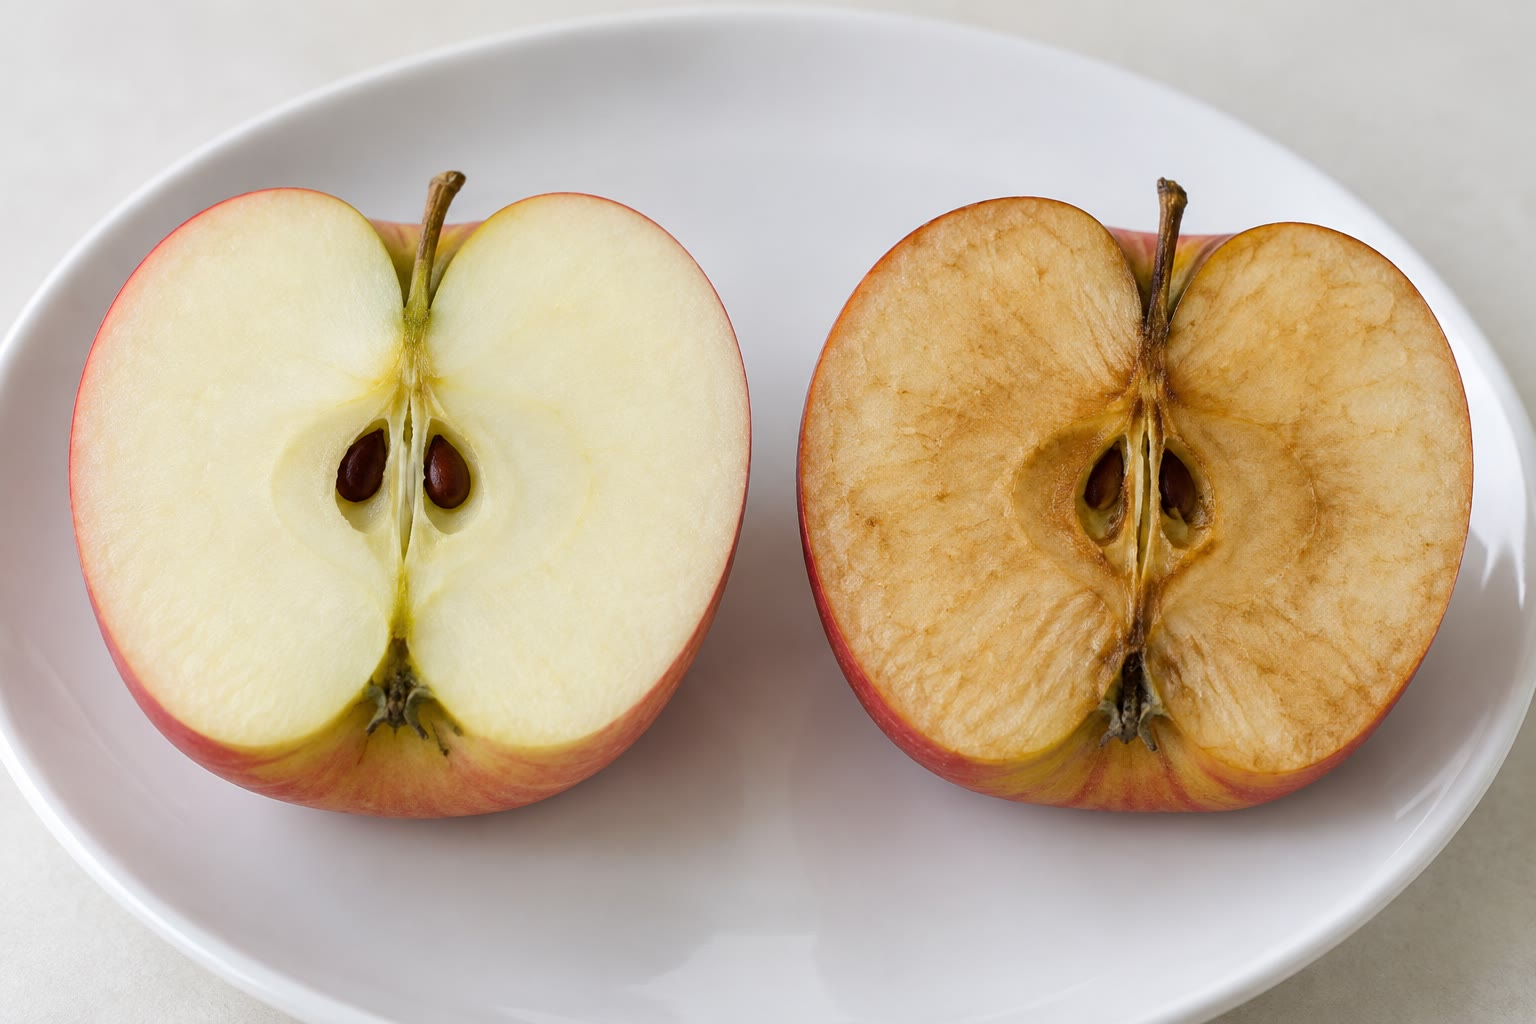
\includegraphics[width=\linewidth,height=4.6cm,keepaspectratio]{images/book1/ai/g5-apple-browning.jpg}

{\small Uma metade fresca e uma metade deixada uma hora no \omterm{def:g4:air-a-mixture-of-gases:air}{ar}.}
\end{minipage}
\end{omfigure}

\begin{omfigure}
\begin{tikzpicture}[font=\small]
  \node[font=\small\bfseries, omDef] at (2.7,4.6) {pode ser desfeita};
  \node[font=\small\bfseries, omProp] at (9.6,4.6) {não pode ser desfeita};
  \draw[black!30] (6.1,4.9) -- (6.1,-0.3);
  % reversible pairs
  \foreach \y/\a/\b in {3.6/{açúcar + água}/{\shortstack{água com\\ açúcar}}, 2.0/{gelo}/{água líquida},
                        0.4/{\shortstack{areia +\\ cascalho}}/{uma mistura}} {
    \node[draw=omDef, fill=omDef!6, rounded corners=2pt, minimum width=2.3cm,
      minimum height=0.8cm] at (0.9,\y) {\a};
    \node[draw=omDef, fill=omDef!6, rounded corners=2pt, minimum width=2.3cm,
      minimum height=0.8cm] at (4.6,\y) {\b};
    \draw[->, thick, omDef] (2.3,\y+0.12) -- (3.25,\y+0.12);
    \draw[<-, thick, omDef] (2.3,\y-0.12) -- (3.25,\y-0.12);
  }
  % irreversible ones
  \foreach \y/\a/\b in {3.6/{ovo cru}/{ovo cozido}, 2.0/{madeira}/{\shortstack{cinza, fumaça,\\ gases}},
                        0.4/{ferro}/{ferrugem}} {
    \node[draw=omProp, fill=omProp!6, rounded corners=2pt, minimum width=2.0cm,
      minimum height=0.8cm] at (7.6,\y) {\a};
    \node[draw=omProp, fill=omProp!6, rounded corners=2pt, minimum width=2.9cm,
      minimum height=0.8cm] at (11.5,\y) {\b};
    \draw[->, thick, omProp] (8.8,\y) -- (9.85,\y);
  }
\end{tikzpicture}

{\small À esquerda: \omterm{def:g5:irreversible-changes:reversible}{transformações reversíveis}; a seta dupla diz que elas
podem ir nos dois sentidos. À direita: \omterm{def:g5:irreversible-changes:chemical-change}{transformações químicas}, num
sentido só.}
\end{omfigure}

\section{Pistas de que apareceu uma substância nova}

\begin{method}[É uma transformação química? Procure as pistas]\label{met:g5:irreversible-changes:clues}
Uma substância nova muitas vezes se denuncia por uma destas pistas:
\begin{enumerate}
  \item uma \textbf{cor} nova (o marrom de uma fatia de pão torrada);
  \item \textbf{bolhas} de um gás aparecendo num líquido sem nenhum
        aquecimento (vinagre despejado sobre bicarbonato de sódio);
  \item um \textbf{cheiro} novo (leite azedo, torrada queimada);
  \item liberação de \textbf{calor ou luz} (uma vela acesa);
  \item um \textbf{sólido que aparece} num líquido límpido, ou grumos que
        se formam (o leite talhando).
\end{enumerate}
Uma pista sozinha pode enganar: a água fervendo faz bolhas, mas nada de
novo é fabricado --- as bolhas são vapor de água, e a água volta quando
o vapor esfria. Procure várias pistas e pergunte: dá para desfazer?
\end{method}

\begin{omfigure}
\begin{tikzpicture}[font=\small]
  \foreach \k/\t in {0/{cor nova}, 1/{bolhas de gás}, 2/{cheiro novo},
                     3/{calor ou luz}, 4/{aparece um sólido}} {
    \begin{scope}[xshift=\k*3.2cm]
      \draw[omProp, line width=0.8pt, fill=omProp!5] (0,0) circle (1.0);
      \node[anchor=north, align=center] at (0,-1.15) {\t};
    \end{scope}
  }
  % 1: colour, a slice of toast half brown
  \fill[yellow!20, draw=brown!60] (-0.55,-0.5) rectangle (0.55,0.55);
  \fill[brown!55] (0,-0.5) rectangle (0.55,0.55);
  % 2: bubbles in a beaker
  \begin{scope}[xshift=3.2cm]
    \pic[transform shape, scale=0.45] at (0,-0.55) {beaker={0.7}{omWater!80}};
    \foreach \x/\y in {-0.15/-0.2,0.1/0.05,-0.05/0.25,0.18/-0.35,-0.2/0.15}
      \draw[black!55] (\x,\y) circle (0.05);
  \end{scope}
  % 3: smell, wavy lines
  \begin{scope}[xshift=6.4cm]
    \foreach \x in {-0.35,0,0.35} \draw[black!55, line width=0.8pt, decorate,
      decoration={snake, amplitude=1.5pt, segment length=6pt}] (\x,-0.6) -- (\x,0.6);
  \end{scope}
  % 4: a flame
  \begin{scope}[xshift=9.6cm]
    \fill[orange!80] (0,-0.6) .. controls (-0.45,-0.05) and (-0.15,0.35) .. (0,0.7)
      .. controls (0.15,0.35) and (0.45,-0.05) .. (0,-0.6);
    \fill[yellow!80] (0,-0.45) .. controls (-0.2,-0.1) and (-0.08,0.15) .. (0,0.3)
      .. controls (0.08,0.15) and (0.2,-0.1) .. (0,-0.45);
  \end{scope}
  % 5: solid settling in a test tube
  \begin{scope}[xshift=12.8cm]
    \pic[transform shape, scale=0.4] at (0,-0.65) {testtube={0.75}{omWater!80}};
    \fill[white, draw=black!40] (-0.08,-0.62) rectangle (0.08,-0.5);
    \foreach \x/\y in {-0.04/-0.3,0.04/-0.1,0/0.1} \fill[black!35] (\x,\y) circle (0.03);
  \end{scope}
\end{tikzpicture}

{\small Cinco pistas de que uma \omterm{def:g5:irreversible-changes:chemical-change}{transformação química} pode ter
acontecido.}
\end{omfigure}

\begin{inthelab}[Vinagre sobre bicarbonato de sódio]
O professor põe uma colher de bicarbonato de sódio, um pó branco, no
fundo de um béquer e despeja um pouco de vinagre. A mistura borbulha e
espuma na hora: um gás é liberado, uma pista de \omterm{def:g5:irreversible-changes:chemical-change}{transformação química}.
Quando o borbulhamento para, o bicarbonato de sódio sumiu e não pode ser
recuperado secando a mistura.
\end{inthelab}

\begin{omfigure}
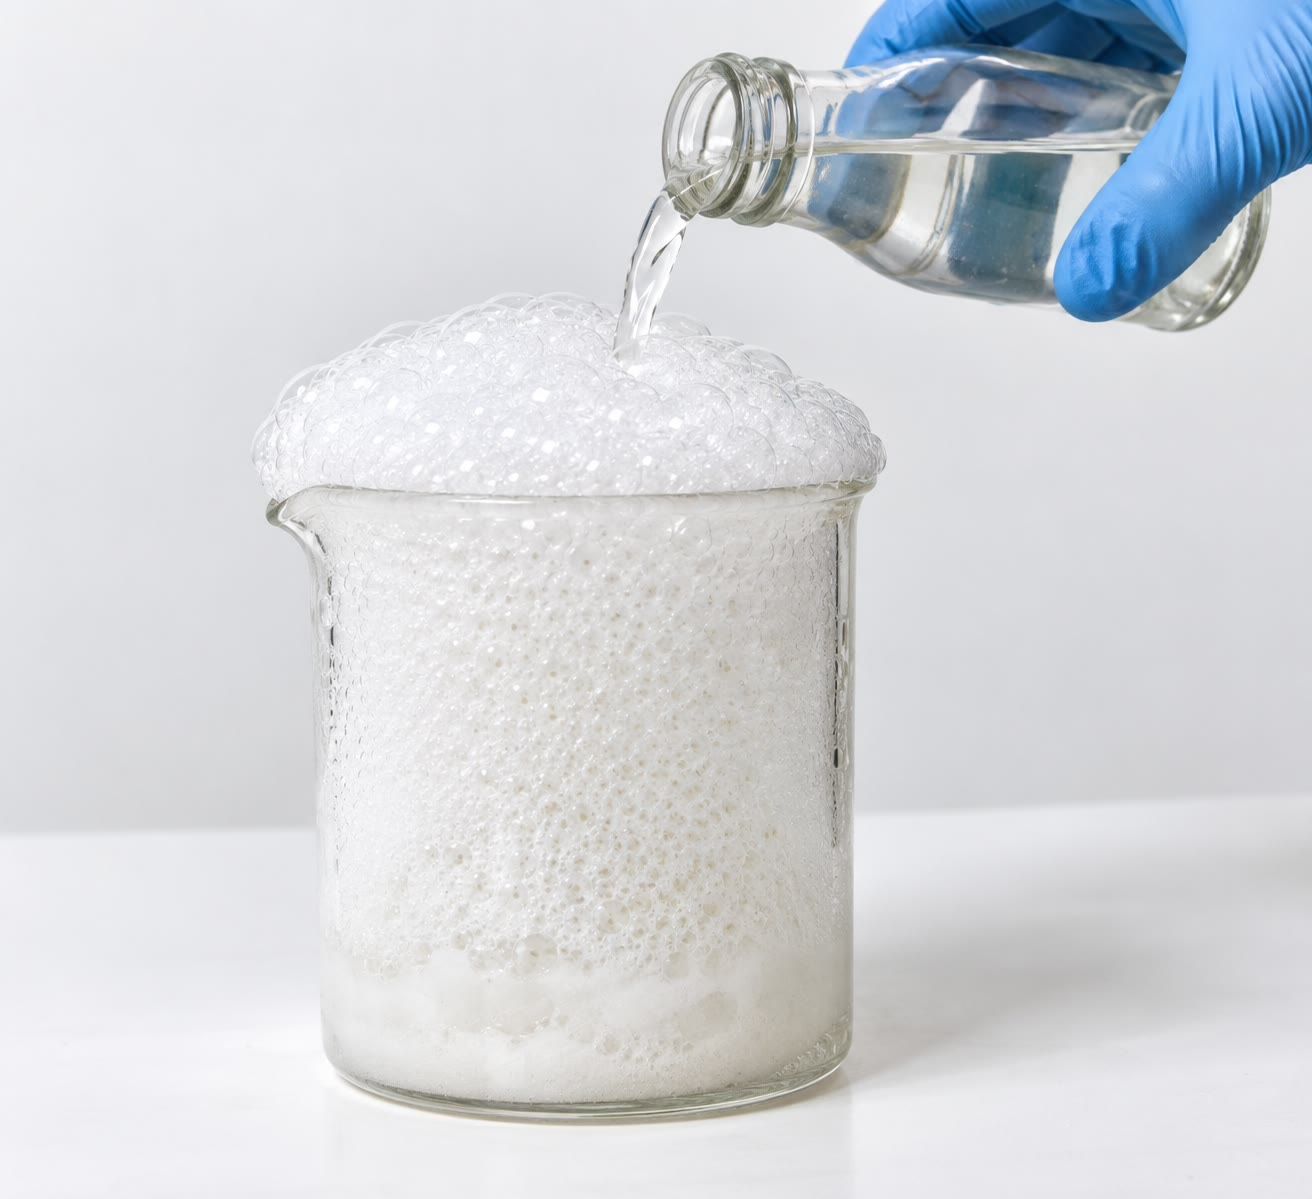
\includegraphics[width=0.5\linewidth]{images/book1/ai/g5-baking-soda-lab.jpg}

{\small Vinagre sobre bicarbonato de sódio: um gás é liberado.}
\end{omfigure}

\section{Transformações úteis e prejudiciais}

\begin{proposition}[Transformações químicas à nossa volta]\label{prop:g5:irreversible-changes:around}
Muitas \omterm{def:g5:irreversible-changes:chemical-change}{transformações químicas} são úteis: cozinhar os alimentos, assar o
pão, queimar gás para aquecer uma casa, o gesso ou o cimento que
endurecem. Outras causam estragos: o ferro que enferruja, a comida que
estraga, a madeira que apodrece. Não podemos desfazê-las, mas podemos
deixá-las mais lentas:
\begin{itemize}
  \item a comida dura mais no frio da geladeira;
  \item uma tinta ou uma película de óleo mantêm o \omterm{def:g4:air-a-mixture-of-gases:air}{ar} e a água longe do
        ferro;
  \item uma maçã cortada regada com suco de limão escurece mais devagar.
\end{itemize}
\end{proposition}

\begin{omfigure}
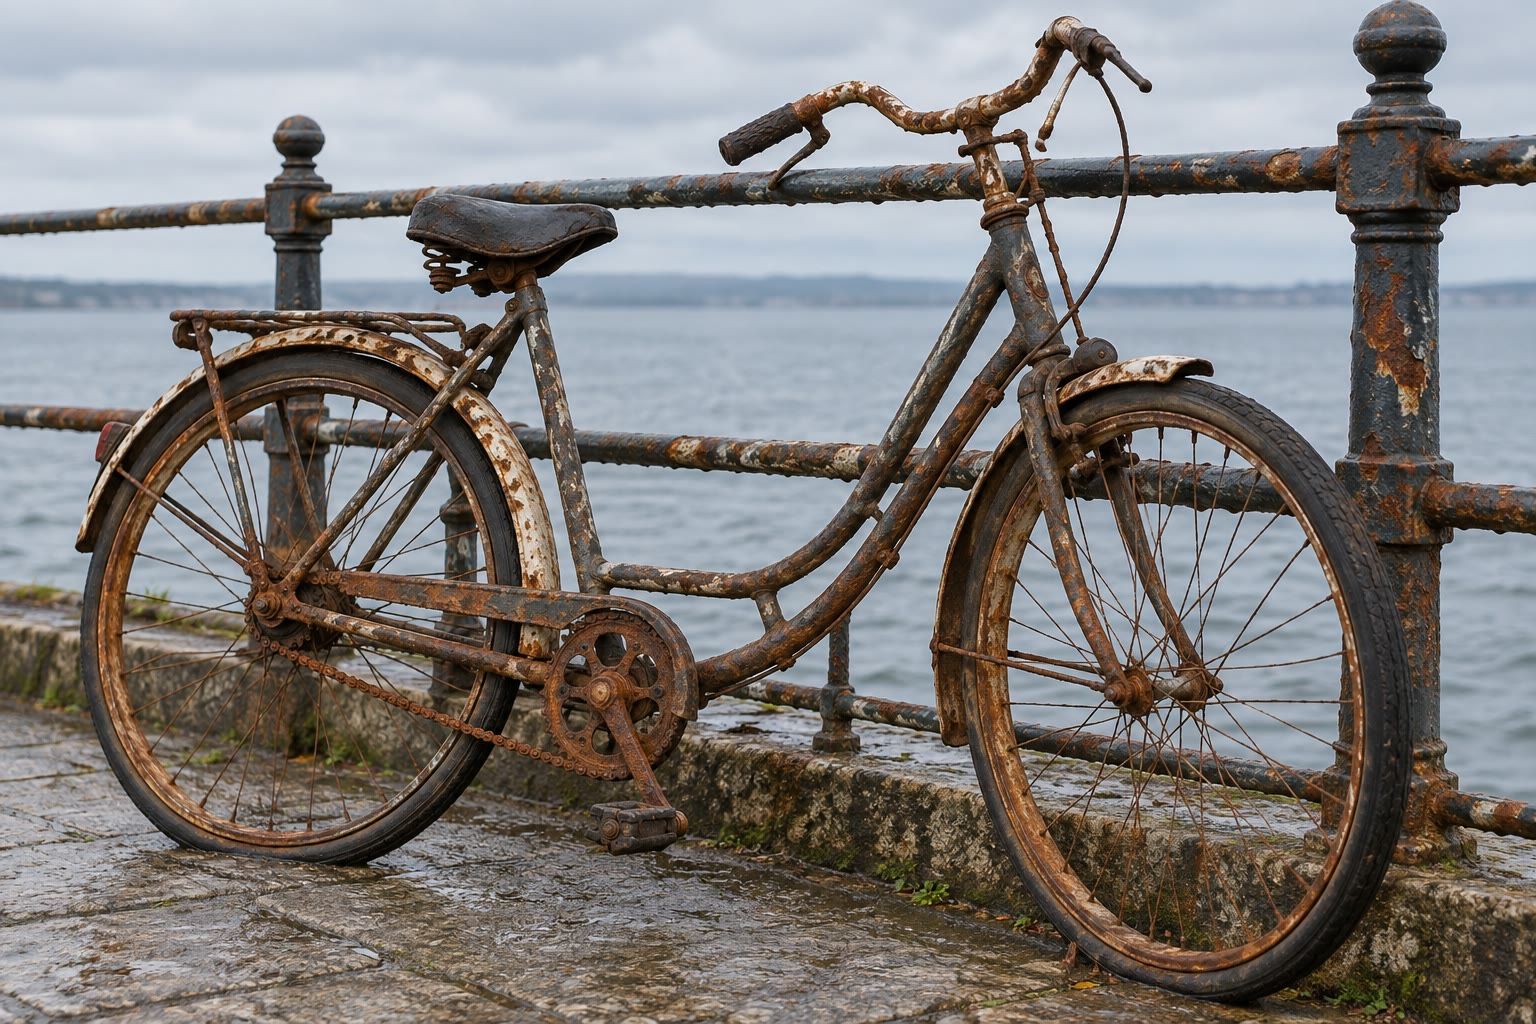
\includegraphics[width=0.55\linewidth]{images/book1/ai/g5-rusty-bicycle.jpg}

{\small Uma bicicleta deixada na chuva durante anos: o ferro
enferrujou.}
\end{omfigure}

\begin{remark}[Desfazer, mas não de um jeito simples]\label{rem:g5:irreversible-changes:not-simply}
``Não pode ser desfeita'' quer dizer que não há um caminho simples de
volta, como esfriar ou secar. Os químicos às vezes conseguem transformar
a ferrugem de novo em ferro, mas só com um forno e com outras
substâncias: isso é uma outra \omterm{def:g5:irreversible-changes:chemical-change}{transformação química}, e não um
desfazer.
\end{remark}

\section{Exercícios}

\begin{exercise}[$\star$]\label{exo:g5:irreversible-changes:1}
Diga se cada transformação pode ser desfeita: derreter chocolate,
queimar um fósforo, \omterm{def:g2:mixing-and-dissolving:dissolve}{dissolver} sal na água, torrar pão.
\end{exercise}

\begin{exercise}[$\star$]\label{exo:g5:irreversible-changes:2}
O que é uma \omterm{def:g5:irreversible-changes:chemical-change}{transformação química}? Dê dois exemplos da cozinha.
\end{exercise}

\begin{exercise}[$\star$]\label{exo:g5:irreversible-changes:3}
Dissolve-se sal na água. Como recuperar o sal? \omterm{def:g2:mixing-and-dissolving:dissolve}{Dissolver} é uma
\omterm{def:g5:irreversible-changes:reversible}{transformação reversível}?
\end{exercise}

\begin{exercise}[$\star$]\label{exo:g5:irreversible-changes:4}
Que pistas de \omterm{def:g5:irreversible-changes:chemical-change}{transformação química} você percebe quando o leite azeda?
Dê duas.
\end{exercise}

\begin{exercise}[$\star$]\label{exo:g5:irreversible-changes:5}
Olhe a figura das duas colunas. Que transformações têm uma seta dupla?
O que a seta dupla quer dizer?
\end{exercise}

\begin{exercise}[$\star$]\label{exo:g5:irreversible-changes:6}
Por que se põe óleo na corrente de uma bicicleta? Que \omterm{def:g5:irreversible-changes:chemical-change}{transformação
química} o óleo deixa mais lenta?
\end{exercise}

\begin{exercise}[$\star$]\label{exo:g5:irreversible-changes:7}
Quando se despeja vinagre sobre bicarbonato de sódio, a mistura
borbulha. Que pista é essa?
\end{exercise}

\begin{exercise}[$\star$]\label{exo:g5:irreversible-changes:8}
Dê uma \omterm{def:g5:irreversible-changes:chemical-change}{transformação química} útil e uma \omterm{def:g5:irreversible-changes:chemical-change}{transformação química}
prejudicial.
\end{exercise}

\begin{exercise}[$\star$]\label{exo:g5:irreversible-changes:9}
Por que guardamos o leite na geladeira?
\end{exercise}

\begin{exercise}[$\star\star$]\label{exo:g5:irreversible-changes:10}
A água faz bolhas quando ferve. Ferver é uma \omterm{def:g5:irreversible-changes:chemical-change}{transformação química}?
Explique por que uma única pista não basta.
\end{exercise}

\begin{exercise}[$\star\star$]\label{exo:g5:irreversible-changes:11}
O Tom diz: ``Quando a vela \omterm{def:g4:what-a-fire-needs:burning}{queima}, a cera só derrete e vai embora, como
o gelo.'' Use duas pistas para explicar por que a \omterm{def:g4:what-a-fire-needs:burning}{queima} de uma vela é
uma \omterm{def:g5:irreversible-changes:chemical-change}{transformação química}, e não só um derretimento.
\end{exercise}
